
\documentclass[aps,prl,reprint]{revtex4-2}
\usepackage{gensymb}
\usepackage{graphicx}
\usepackage{amsmath}
\usepackage{hyperref}
\usepackage{dsfont}
\usepackage{relsize}
\usepackage{wrapfig}
\usepackage{graphicx}
\usepackage{hyperref}
\hypersetup{colorlinks=true, citecolor=blue, urlcolor=blue, linkcolor=blue}


\begin{document}

% Use the \preprint command to place your local institutional report
% number in the upper righthand corner of the title page in preprint mode.
% Multiple \preprint commands are allowed.
% Use the 'preprintnumbers' class option to override journal defaults
% to display numbers if necessary
%\preprint{}

%Title of paper
\title{AFT Lab}

% repeat the \author .. \affiliation  etc. as needed
% \email, \thanks, \homepage, \altaffiliation all apply to the current
% author. Explanatory text should go in the []'s, actual e-mail
% address or url should go in the {}'s for \email and \homepage.
% Please use the appropriate macro foreach each type of information

% \affiliation command applies to all authors since the last
% \affiliation command. The \affiliation command should follow the
% other information
% \affiliation can be followed by \email, \homepage, \thanks as well.
\author{Trevor Smith, Alex Storrer}
\email[]{smith.tr@northeastern.edu}
\homepage[]{https://github.com/trevorm4x/}
%\thanks{}
%\altaffiliation{}
\affiliation{Northeastern University}


\date{\today}

\begin{abstract}
	Nothing is here
\end{abstract}


\maketitle

% body of paper here - Use proper section commands
% References should be done using the \cite, \ref, and \label commands
\section{Introduction}
% The Introduction should contain 1 or 2 paragraphs.
% Briefly state the physics underlying the experiment
% (what is being tested and why). 
Fourier analysis is the practice of viewing a time-domain signal in the
frequency domain. Named after the mathemetician Joseph Fourier for his 
breakthrough discovery that most functions, even discontinuous functions
like the step function, can be represented as an infinite sum of sine 
waves, the advancement was originally made in pursuit of more easily
solving complex differential equations describing heat transfer. Some 
scientists and engineers, however, do Fourier wrong by simply
referring to the technique by the anagram of its modern discrete 
implementation, by saying, for example, ``plot the FFT". \\

The FFT, short for Fast-Fourier Transform, is as stated a method for
calculating the discrete Fourier transform of a finite time-domain signal.
One can forgive those who refer to Fourier analysis generally as ``FFT", 
considering how this ingenious algorithm has paved the way for
the discrete Fourier transform's widespread usage in signal processing
across a wide range of fields and disciplines. \\

Utilizing a divide-and-conquer technique, the FFT could be compared to 
a sailboat that, rather than following the wind directly to its destination,
turns sharply to the side and tacks back and forth across the wind,
taking a significantly longer and more complicated path that arrives in 
a fraction of the time. To understand just how well this analogy works,
consider that the first step the FFT performs on a signal of length 2049
is to add another 2047 zeros onto the end so that the signal length is 
an exact power of 2. \\

In this lab we will be conducting Fourier analysis, with the help of the 
FFT algorithm, of various acoustic signals. This analysis is particularly
interesting in the context of speech and musical instruments, as noised that
to our ears may sound like ``one" note or vowel sound are in fact more
often than not rich with multiple harmonics throughout the frequency spectrum.\\

We will first conduct a simplified test implemented entirely in software,
examining the effect of longer observations on the linewidth, or uncertainty
in the frequency domain, numerically. We will then conduct a simple test
using an function generator with an oscilloscope to collect data for a 
sine wave and square wave, in order to compare their frequency responses. \\

In the next phase of the lab, acoustic signals will be examined. 
First, we will explore the interaction of two tuning forks as they 
constructively and destructively interfere due to slight differences 
in their frequency, producing what is known as a ``beat". We will then
explore characteristics of musical notes produced by a whistling sound, 
the human voice producing vowel sounds, and musical instruments. \\

Finally, we will conduct a numerical exploration of the breakdown of accurate
signal reconstruction in the time-domain as a function of the nyquist
frequency and the fundamental frequency of the signal. 

\section{Apparatus}
% List equipment components (manufacturer, model
% numbers and brief specifications). 

The apparatus consisted of the following.
\begin{itemize}
\end{itemize}

\section{Basic FFT}
% Briefly describe the experimental procedures (in your own words, but don’t overdo it)
% Discuss calibrations, etc., if required
% Include necessary equations and put them on their own line (number them, e.g. “Eq. (3)”)
% Include plots showing relevant results (label each figure, e.g. “Fig. 3”, with caption).
% Describe what you found (describe what the plot illustrates)

\subsection{Procedure and Results}

In this section, a time-vector from 0 to 0.1 using 2048 equally spaced points
was produced, and used to build a sine wave of equation $y=sin(2\pi 100 x)$, 
shown in \ref{shortsine_TD}.
The signal was then transformed into the frequency domain, using the 
FFT algorithm. With this signal, as with all signals for the duration of the
lab, the signal was multiplied by a hamming window before performing the
discrete Fourier transform to mitigate spectral leakage. \\


\begin{figure}[h]
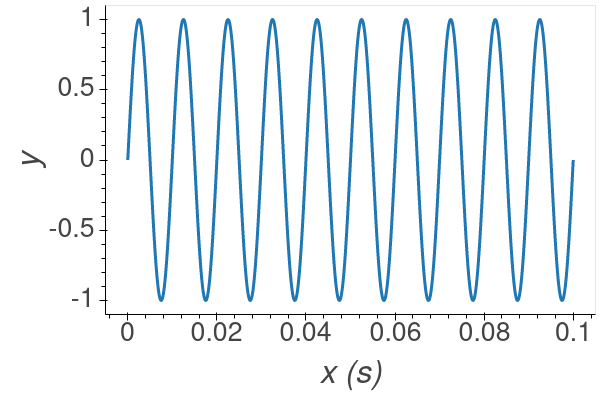
\includegraphics[width=0.34\textwidth]{../Images/l5_A_1a.png}
\caption{\label{shortsine_TD} Sine wave of frequency 100 Hz, observed for 0.1 seconds.}
\end{figure}

The Fourier analysis produced the expected frequency of 100 Hz, verifying that
the technique was applied correctly, as seen in \ref{shortsine_FD}. 

\begin{figure}[h]
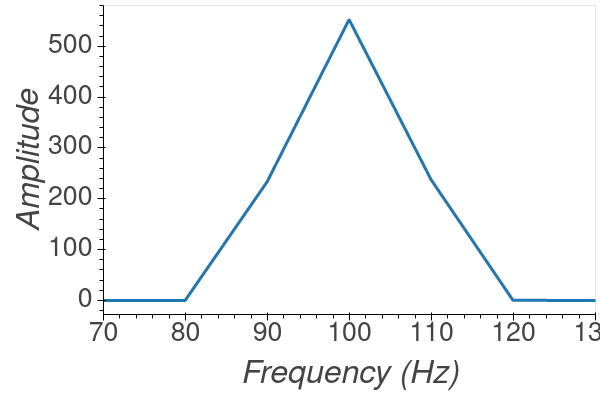
\includegraphics[width=0.34\textwidth]{../Images/l5_A_1b.png}
\caption{\label{shortsine_FD} Sine wave of frequency 100 Hz, observed for 0.1 seconds, in the frequency domain.}
\end{figure}

A second sine signal, calculated with the same sine function and N samples
but longer observation window of 1 second, was produced, as seen in 
\ref{longsine_TD}.

\begin{figure}[h]
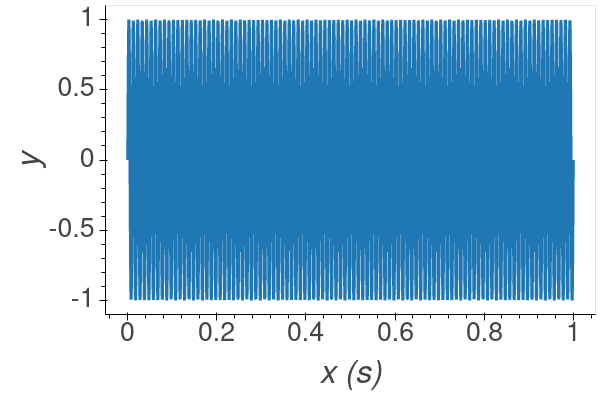
\includegraphics[width=0.34\textwidth]{../Images/l5_A_2a.png}
\caption{\label{shortsine_TD} Sine wave of frequency 100 Hz, observed for 1.0 seconds.}
\end{figure}

This longer sine wave was analyzed in the frequency domain as well, producing
a 100 Hz peak, as seen in \ref{longsine_FD} with the same x-axis range as 
\ref{shortsine_FD}.

\begin{figure}[h]
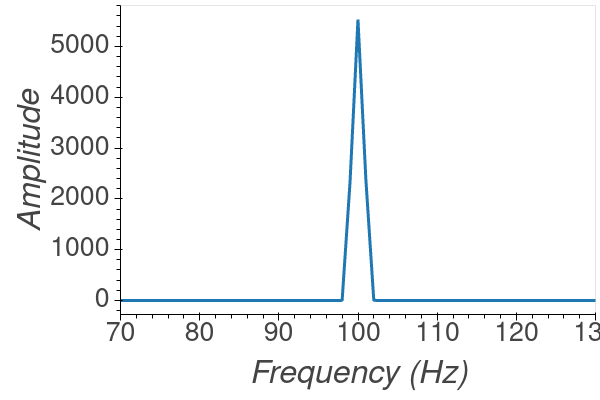
\includegraphics[width=0.34\textwidth]{../Images/l5_A_2b.png}
\caption{\label{shortsine_TD} Sine wave of frequency 100 Hz, observed for 1.0 seconds, in the frequency domain.}
\end{figure}

The characteristics of these two alike signals can be easily compared in 
\ref{comparisine_FD}, however quantitative characteristics are also given in 
\ref{comparisine_TB}. 

\begin{figure}[h]
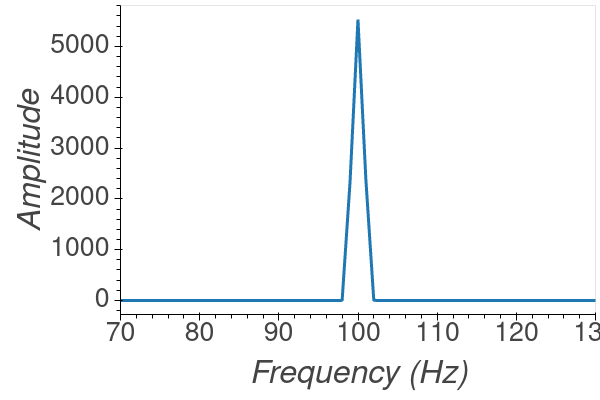
\includegraphics[width=0.34\textwidth]{../Images/l5_A_2b.png}
\caption{\label{comparisine_FD} Comparison of the short (0.1 second) and long
(1.0 second) sine waves, given by the same equation, using Fourier analysis.}
\end{figure}

\subsection{Conclusion}

Uncertainty in the frequency of a signal, which manifests as the linewidth
of a peak in the frequency domain, is reduced as a function of observation time.
This is the result of a flavor of the Heisenberg Uncertainty Principle, where 
longer observations (greater N cycles) of a signal trade better certainty of 
the location of the signal in the frequency domain for worse certainty of the 
location of the signal in the time domain. \\

This simple experiment confirms that linewidth $\Gamma$ is reduced with
longer observations or more cycles. A higher precision FFT was produced
in this experiment by collecting 100 cycles than by collecting 10 cycles.
It also shows that if a longer observation time is used while the number
N of samples is kept constant, sample rate decreases, which is seen in the
frequency range as well. It is important to note that although the 
resolution of the frequency spectrum was reduced by a factor of ten (larger frequency
bins), the uncertainty or linewidth was still reduced. 

\begin{widetext}
\begin{center}
\begin{table}[t]
\renewcommand{\arraystretch}{1}
\setlength{\tabcolsep}{10pt}
\caption{\label{comparisine_TB} Frequency response and parameters given by a
short and long observation of the same sine equation.}
\begin{tabular}{|c|c|c|c|c|c|}
%\hline
\toprule
Time (s) & Cycles M & Samples N & FFT Range $\Delta f$ & Resolving Power $\frac{f_0}{\delta f}$ (Hz) & Linewidth $\Gamma$ (Hz) \\
\colrule
0.1  &  10   &  2048  &  10225   & 10.00 &  17.4 \\ \colrule
1.0  &  100  &  2048  &  1022.5  & 1.000 &  1.74 \\ \hline
\botrule
\end{tabular}
\end{table}
\end{center}
\end{widetext}

%--------------------------------------------------------------------%
%  It should be noted that after this point are reference functions  % 
%--------------------------------------------------------------------%


\subsection{Results}

\newpage
\begin{equation}
    \mathlarger{\eta_{PV}}=P_E/P_L
    \label{eta_PV}
\end{equation}

\subsection{Conclusions}

\section{Summary}

\begin{widetext}
\begin{center}
\begin{table}[h]
\renewcommand{\arraystretch}{1.35}
\setlength{\tabcolsep}{10pt}
\caption{\label{}Measured and accepted values of the speed of light and refractive index of various materials.}
\begin{tabular}{|c|c|c|c|c|}
%\hline
\toprule
Apparatus &  $\eta$ (\%) & Accepted $\eta$ value & Refs. & Deviation \\
\colrule
Photovoltaic Cell &  $15 \pm 2$ & $17 \pm 2.5$ & \cite{Solar Cell} & $0\sigma$  \\
\colrule
Elecrolyzer &  $87 \pm 6$ & 80 & \cite{Electrolyzer} & $2\sigma$  \\
\colrule
Hydrogen Fuel Cell &  $49 \pm 5$ & 60 & \cite{Fuel Cell} & $-3\sigma$  \\
%\hline
\botrule
\end{tabular}
\end{table}
\end{center}
\end{widetext}





\begin{thebibliography}{9}
%
\bibitem{HHV} 
Wikipedia, Heat of Combustion: \\
\href{https://en.wikipedia.org/wiki/Heat_of_combustion}{https://www.wikepedia.com}
%
\bibitem{Solar Cell} 
Energysage, Most Efficient Solar Panels\\
\href{https://news.energysage.com/what-are-the-most-efficient-solar-panels-on-the-market/#:~:text=How%20efficient%20are%20solar%20panels,are%20not%20above%2020%25%20efficiency.}{https://www.energysage.com/}
%
\bibitem{Electrolyzer} 
Carbon Commentary, Hydrogen made by Electolysis\\
\href{https://www.carboncommentary.com/blog/2017/7/5/hydrogen-made-by-the-electrolysis-of-water-is-now-cost-competitive-and-gives-us-another-building-block-for-the-low-carbon-economy}{https://www.carboncommentary.com}
%

%
\bibitem{Fuel Cell} 
Energy.gov, Fuel Cell Fact Sheet\\
\href{https://www.energy.gov/sites/prod/files/2015/11/f27/fcto_fuel_cells_fact_sheet.pdf}{https://www.energy.gov}

\end{thebibliography}


\end{document}
%
% ****** End of file apstemplate.tex ******

